\documentclass[11pt,letter]{article}
\usepackage[top=1.00in, bottom=1.0in, left=1.1in, right=1.1in]{geometry}
\renewcommand{\baselinestretch}{1.1}
\usepackage{graphicx}
\usepackage{natbib}
\usepackage{amsmath}
\usepackage{amssymb} 
\usepackage{hyperref}
\usepackage{xr-hyper}
\externaldocument{decsens_supp}
% \usepackage{hyperref}

\def\labelitemi{--}
\parindent=0pt
\begin{document}

\title{A simple explanation for declining temperature sensitivity \\ with warming} % The illusion of declining temperature sensitivity with warming // Sensitivities are not declining with warming OR As climate change accelerates biology, chasing statistical artifacts ensues
\author{E. M. Wolkovich$^{1,a}$,  J. Auerbach$^{2}$, C. J. Chamberlain$^{3}$, D. M. Buonaiuto$^{3}$, \\ A. K. Ettinger$^4$, I. Morales-Castilla$^{5}$ \& A. Gelman$^{2}$} 

\date{\today} 
\maketitle
$^1$Forest \& Conservation Sciences, Faculty of Forestry, University of British Columbia, Vancouver, British Columbia, Canada\\
$^2$Department of Statistics, Columbia University, New York, NY 10027, USA\\
$^3$Department of Organismic and Evolutionary Biology, Harvard University, Cambridge, Massachusetts, USA\\
$^4$TNC, USA\\
$^5$Department of Life Sciences, University of Alcal\`a CTRA N-II, KM., 33,600, 28802, Alcal\`a de Henares, Spain\\
$^a$Corresponding author.


\begin{abstract} % 140 plus cites
Temperature sensitivity---the magnitude of a biological response per $^{\circ}$C---is a fundamental concept across scientific disciplines, especially biology, where temperature determines the rate of many plant, animal and ecosystem processes. Recently, a growing body of literature in global change biology has found temperature sensitivities decline as temperatures rise \citep{fu2015,gusewell2017,piao2017,dai2019ag}. Such observations have been used to suggest climate change is reshaping biological processes, with major implications for forecasts of future change. Here we present a simple alternative explanation for observed declining sensitivities: the use of linear models to estimate non-linear temperature responses. Corrections for the non-linearity of temperature response in simulated data and long-term phenological data from Europe remove the apparent decline. Our results show that rising temperatures combined with linear estimates based on calendar time are expected to produce observations of declining sensitivity---without any shift in the underlying biology.
\end{abstract}
% Recently, a growing body of literature in global change biology has found temperature sensitivities decline as temperatures rise \citep{fu2015,gusewell2017,piao2017,dai2019ag}. These declines are generally attributed to shifts in underlying biological processes caused by warming, yet to date there is no clear evidence of mechanistic changes.

\newpage
\section{Main text} % 981 right now
Climate change has reshaped biological processes around the globe, with shifts in the timing of major life history events (phenology), carbon dynamics and other ecosystem processes \citep{IPCC:2014sm}. With rising temperatures,  a growing body of literature has documented changes in temperature sensitivity---the magnitude of a biological response scaled per $^{\circ}$C. Many studies have found declining responses to temperature in recent decades \citep{fu2015,gusewell2017,piao2017,dai2019ag}, and some have reported more uniform sensitivities across elevation \citep{vitasse2018}, or lower sensitivities in warmer, urban areas \citep{meng2020}.\\

Most studies attribute changes in temperature sensitivity to shifts in underlying biological processes. For example, researchers have suggested weaker temperature sensitivities are evidence of increased light limitation in the tundra \citep{piao2017}, or a decline in the relative importance of warm spring temperatures for spring phenological events (e.g., leafout, insect emergence) in the temperate zone \citep{fu2015, meng2020}, as other evironmental triggers (e.g., winter temperatures that determine `chilling') play a larger role. Yet, despite an increase in studies reporting declining or shifting temperature sensitivites, none have provided strong evidence of the biological mechanisms underlying these changes  \citep[e.g.,][]{fu2015,meng2020}. The missing mechanisms may be hidden in the data: environmental factors moderate biological processes in complex ways \citep{chuine2016,gusewell2017}, are strongly correlated in nature \citep[e.g.,][]{fu2015}, and temperature variance shifts over time and space \citep{keenan2019}. \\
%  fundamental science suggests that warm spring temperatures are the main controller of many temperate phenological events (e.g., leafout, insect emergence), but winter temperatures and photoperiod can also determine the timing of events. Thus, an increased role of winter temperatures or photoperiod could explain observed declines in the temperature sensitivity of plant phenology with warming. 
% ... fundamental science predicts declines in the temperature sensitivity of temperate plant phenology, as the role of spring temperature diminishes relative to the increasing importance of winter temperatures and daylength... For example, the temperature sensitivity of spring leafout may decline if warmer winters mean plants fail to receive enough winter chilling.  

Here we propose a simpler alternative expanation: the use of linear models for non-linear responses to temperature. Researchers generally use methods with assumptions of linearity to calculate temperature sensitivities, often relying on some form of linear regression to compute a change in a quantity---days to leafout or carbon sequestered over a fixed time, for example---per $^{\circ}$C, thus ignoring that many biological responses to temperature are non-linear. We show, theoretically then with simulated and empirical data, how the use of linear methods for non-linear processes can produce an illusion that the mechanisms underlying biological processes are changing.\\ % We demonstrate this theoretically using first-hitting-time models---and empirically---using both simulated data and long-term phenological data from Europe.\\

Many observed biological events are the result of continuous non-linear processes that depend on temperature, which are discretized into temporal units for measurement. For example, a biological response, such as leafout, occurs when a certain thermal sum is reached, and plants will reach this threshold more quickly---in calendar time---when average daily temperatures are warmer. Biologically, however, the plants may require the same temperature sum. Indeed any process observed or measured as the time until reaching a threshold is inversely proportional to the speed at which that threshold is approached. Temperature determines the speed of many biological processes. Thus, at very low temperatures plants would never leaf out and at higher temperatures they could leaf out in only a matter of days---yet sensitivities estimated from linear regression at higher (warmer) temperatures would appear much lower than those observed at lower temperatures. Warming acts to step on the biological accelerator, and thus may produce declining sensitivities without any change in the underlying process.  \\ % Warming acts to step on the biological accelerator and makes the use of classic calendar time precarious
% calendar time is the same, but the biological time is much greater
% amount of change that can occur in a day depends on temperature

We show this by deriving the relationship between a biological response and temperature using simple stochastic model, which describes the first time a random process hits a threshold (see `A first-hitting-time model of leafout' in SI). Our model holds the temperature threshold for leafout constant. Even though the mechanism by which temperature leads to leafout does not change, the model produces declining sensitivity---as measured in days per $^{\circ}$C---with warming. Indeed, under this model constant temperature sensitivity would be evidence that the temperature threshold is not constant and the mechanisms underlying the leafout process have changed. \\ % We consider two common scenarios: one measuring average daily temperature up until the leafout date, and the other measuring average daily temperature over a fixed window (such as March 1st to April 30th). 

Simulations show that correcting for non-linearity removes apparent declines in temperature sensitivity (Fig. \ref{fig:basicsimswpep}, \ref{fig:basicsims}, \href{https://github.com/temporalecologylab/labgit/tree/master/projects/decsenspost}{code link}). Assuming a model where warming increases the required thermal sum for a biological event---a common hypothesis for declining sensitivities in spring phenological events---yields declining sensitivities that remain after correcting for non-linearity (Fig. \ref{fig:simsshiftcues}). \\

Further, after correcting for non-linearity in long-term leafout data from Europe, we find little evidence for declining sensitivities with warming (Figs. \ref{fig:basicsimswpep}, \ref{fig:pepper10yr}, \ref{fig:pepper20yr}). An apparent decline in sensitivity for silver birch (\emph{Betula pendula}) from -4.3 days/$^{\circ}$C to -3.6 days/$^{\circ}$C from 1950-1960 compared to 2000-2010 disappears using a log-log regression (-0.17 versus -0.22). We see similar corrections using 20-year windows, and a potential increase in sensitivity for European beech (\emph{Fagus sylvatica}, see Tables \ref{tab:pep10yr}-\ref{tab:pep20yr}). Moreover, the variance of the leafout dates of both species declines as temperatures rise---(declines of roughly 50\%, see Tables \ref{tab:pep10yr}-\ref{tab:pep20yr}), which is expected under our model as warming accelerates towards the thermal threshold that triggers leafout \citep[and in contrast to predictions from changing mechanisms, see][]{ford2016}. \\

Our theoretical model and empirical results show that rising temperatures are sufficient to explain declining temperature sensitivity. It is not necessary to invoke changes to the mechanisms that underlie the biological processes themselves. \\

% Before anthropogenic climate change, the use of sensitivities calculated from linear models may have been less prone to yielding notable temporal patterns. With warming declining sensitivities should be the null model for analyses using simple linear regressions, and highlights how the nonstationarity of climate change upends methods and approaches that may work in stationary systems \citep{Milly:2008yu,tempeco}.  Attempts to use sensitivities to identify shifting biological process across space has always required caution \citep[e.g.,][]{tansey2017}, but climate change adds further complexity. \\ % Phillimore2012

Inferring biological processes from statistical artifacts is not a new problem \citep[e.g.,][]{nee2005}, but climate change provides a new challenge in discerning mechanism from measurements because it affects biological time, while researchers continue to use calendar time. Other fields focused on temperature sensitivity often use approaches that acknowledge the non-linearity of responses \citep[e.g.,][]{yuste2004}. Researchers have called for greater use of process-based models \citep{keenan2019}, which often include non-linear responses to temperature, but rely themselves on exploratory methods and descriptive analyses for progress \citep{chuine2016}. The challenge, then, is to interrogate the implicit and explicit models we use to interpret data summaries, and to develop null expectations that apply across biological and calendar time. \\
% But many fields, still lack the underlying mechanistic understanding to robustly develop and fit process-based models, with many parameters and aspects of the model specification unknown \citep{chuine2016}. Thus we expect more exploratory methods, such as regression, will continue to inform science, but findings from such methods must be interrogated---confronted with multiple diverse methods of calculating similar metrics, tested for logical outcomes, and compared against null models based on biological time. % Greater use of data simulation and null models can highlight issues and bring greater focus on mechanisms. 

\emph{Acknowledgements:} Thanks to TJ Davies, TM Giants, D. Lipson, C. Rollinson, and others. 

\bibliographystyle{..//refs/bibstyles/amnat.bst}
\bibliography{..//refs/decsens.bib}


\newpage
\section* {Figures}

\begin{figure}[h!]
\centering
\noindent 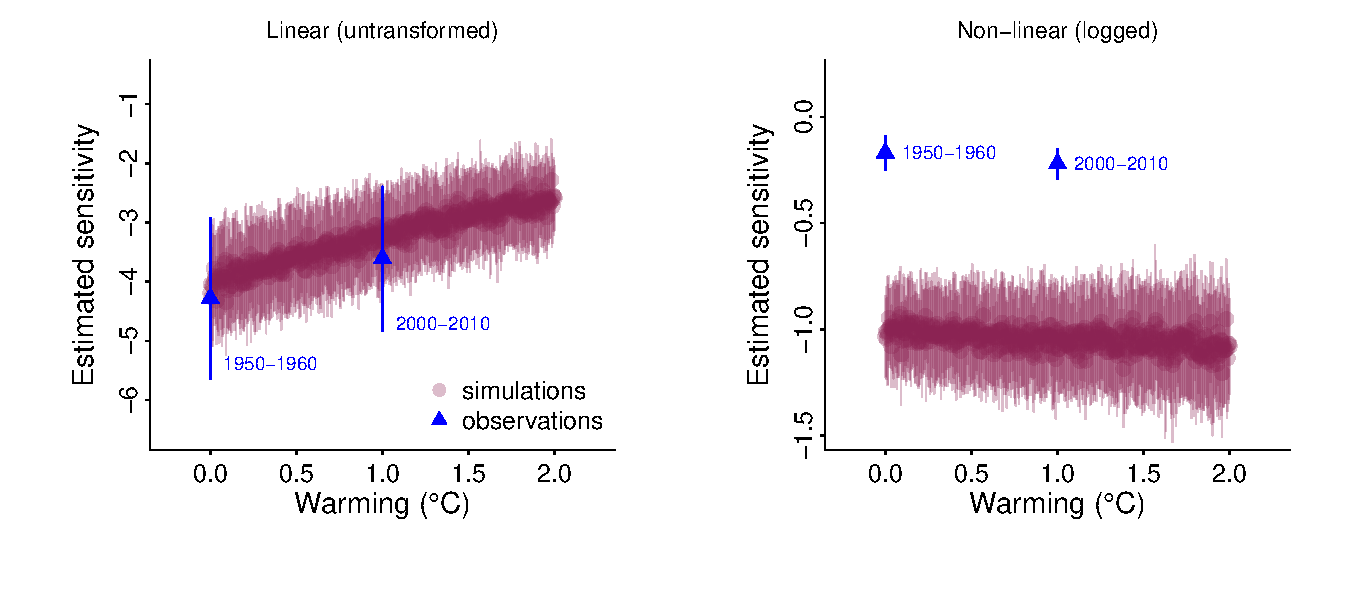
\includegraphics[width=1.05\textwidth]{..//analyses/figures/basicsimsandpepalt.pdf} % 136 words
\caption{\textbf{Shifts in temperature sensitivities with warming occur when using linear models for non-linear processes.} Estimated sensitivities decline with warming in simulations (left) with no underlying change in the biological process when sensitivities were estimated with linear regression (estimated across 45 sites with a base temperature of normal(6,4)). This decline disappears when performing the regression on logged predictor and response variables (right). Such issues may underlie declining sensitivities calculated from observational data, including long-term observations of leafout across Europe (`observations,' using data for \emph{Betula pendula} from PEP725 from for the 45 sites that had complete data for 1950-1960 and 2000-2010), which show a lower sensitivity with warming when calculated on raw data, but no change in sensitivity using logged data. Symbols and lines represent means $\pm$ standard deviations of regressions across sites. See SI for a discussion of why estimated sensitivities are -1 or lower in non-linear models.} % Estimates of sensitivities from logged variables were generally much lower than -1, suggesting other factors or a better metric of temperature underlie leafout dates.
\label{fig:basicsimswpep} % decsensSims.R
\end{figure}


\end{document}


\section{Outline \& notes}

Need to work on this, notes to date on % \href{https://github.com/lizzieinvancouver/decsens/wiki/Statistical-artifacts-in-sensitivities}{here}.\\

\emph{Meeting with Jonathan Auerbach \& Andrew Gelman on 18 December 2019:} 

Fundamental issue is that we have a non-linear relationship ($y=1/x$) being described by a linear function ($y=x$), where $x$ is the mean temp and 1 could be the GDD. The time until you reach a threshold is inversely proportional to the speed you go at. So, at very low temperatures plants would (theoretically) never leaf out and at 200 C days it would take one day. \\

The classic algebra example (they tell me) is how long does it take to drive 200 miles? It depends on your miles per hour. (Side note by Lizzie while typing up these notes: the speed analogy is sort of nice, climate change is stepping on the accelerator, making this algebra problem relevant.)

\begin{itemize}
\item The artifact comes from the mean getting larger while the variance goes down (I think, I may have this noted wrong, but it's about the mean relative to the variance, not just the variance or the mean). If you make the variance scale with the mean you will see the issue go away (though Andrew pointed out this should be done on the $SD$ scale, not the $var$).
\item ``The statistical artifact is that fitting a linear regression requires linearity''said  Jonathan Auerbach.
\item If this was all simple, we could fix it two ways: percent scale (decline relative to some base C temp) or log both axes. (Note from Lizzie: but we don't know when to start accumulating so not sure how this works, though Jonathan seemed to have insight into this.)
\item An example of inferring process from an artifact is regression to the mean, though Andrew pointed out regression to the mean is more complicated compared to this as regression to the mean is a statistical issue and this is just a deterministic reality. 
\item Convexity in economics has had similar problems to this. 
\end{itemize}

\section{Literature notes}

Sagarin 2001: False estimates of the advance of spring (leap year issues). \\

I noticed as you go back to 2014 and before in my ISI searches, you get a lot of soil respiration lit. And in that literature they use $Q_{10}$ for temperature sensitivities, ``[t]he temperature sensitivity of soil respiration is often expressed as the Q10 value; that is, the factor by which soil respiration increases by a 10°C increase in temperature (e.g., Kirschbaum, 1995; Van't Hoff, 1898),'' which would avoid a good dose of the issue we're seeing.\\  % definition from https://agupubs.onlinelibrary.wiley.com/doi/full/10.1002/2017GB005644
% Van't Hoff, J. H. (1898). Lectures on theoretical and physical chemistry. In Chemical Dynamics Part I (pp. 224–229). London: Edward Arnold.

Shen et al. 2014 shows earlier-season vegetation more temperature-sensitive, which is the same artifact. Do we want to work this in?
